%%%%%%%%%%%%%%%%%%%%%%%%%%%%%%%%%%%%%%%%%
% Beamer Presentation
% LaTeX Template
% Version 1.0 (10/11/12)
%
% This template has been downloaded from:
% http://www.LaTeXTemplates.com
%
% License:
% CC BY-NC-SA 3.0 (http://creativecommons.org/licenses/by-nc-sa/3.0/)
%
%%%%%%%%%%%%%%%%%%%%%%%%%%%%%%%%%%%%%%%%%

%----------------------------------------------------------------------------------------
%	PACKAGES AND THEMES
%----------------------------------------------------------------------------------------

\documentclass{beamer}

\mode<presentation> {

% The Beamer class comes with a number of default slide themes
% which change the colors and layouts of slides. Below this is a list
% of all the themes, uncomment each in turn to see what they look like.

%\usetheme{default}
%\usetheme{AnnArbor}
%\usetheme{Antibes}
%\usetheme{Bergen}
%\usetheme{Berkeley}
%\usetheme{Berlin}
%\usetheme{Boadilla}
%\usetheme{CambridgeUS}
%\usetheme{Copenhagen}
%\usetheme{Darmstadt}
%\usetheme{Dresden}
%\usetheme{Frankfurt}
%\usetheme{Goettingen}
%\usetheme{Hannover}
%\usetheme{Ilmenau}
%\usetheme{JuanLesPins}
%\usetheme{Luebeck}
\usetheme{Madrid}
\usepackage{pbox}
\usepackage{listings}
\lstset{language=Java,
                basicstyle=\footnotesize\ttfamily,
                keywordstyle=\footnotesize\color{blue}\ttfamily,
}

%\usetheme{Malmoe}
%\usetheme{Marburg}
%\usetheme{Montpellier}
%\usetheme{PaloAlto}
%\usetheme{Pittsburgh}
%\usetheme{Rochester}
%\usetheme{Singapore}
%\usetheme{Szeged}
%\usetheme{Warsaw}

% As well as themes, the Beamer class has a number of color themes
% for any slide theme. Uncomment each of these in turn to see how it
% changes the colors of your current slide theme.

%\usecolortheme{albatross}
%\usecolortheme{beaver}
%\usecolortheme{beetle}
%\usecolortheme{crane}
%\usecolortheme{dolphin}
%\usecolortheme{dove}
%\usecolortheme{fly}
%\usecolortheme{lily}
%\usecolortheme{orchid}
%\usecolortheme{rose}
%\usecolortheme{seagull}
%\usecolortheme{seahorse}
%\usecolortheme{whale}
%\usecolortheme{wolverine}

%\setbeamertemplate{footline} % To remove the footer line in all slides uncomment this line
%\setbeamertemplate{footline}[page number] % To replace the footer line in all slides with a simple slide count uncomment this line

%\setbeamertemplate{navigation symbols}{} % To remove the navigation symbols from the bottom of all slides uncomment this line
}

\usepackage{graphicx} % Allows including images
\usepackage{booktabs} % Allows the use of \toprule, \midrule and \bottomrule in tables
\usepackage{framed}

%----------------------------------------------------------------------------------------
%	TITLE PAGE
%----------------------------------------------------------------------------------------

\title[Generici e Collezioni]{Generici e Collezioni} % The short title appears at the bottom of every slide, the full title is only on the title page

\author{Claudio Menghi} % Your name
\institute[Polimi] % Your institution as it will appear on the bottom of every slide, may be shorthand to save space
{
Politecnico di Milano \\ % Your institution for the title page
\medskip
\textit{claudio.menghi@polimi.it} % Your email address
}
\date{\today} % Date, can be changed to a custom date

\begin{document}

\begin{frame}
\titlepage % Print the title page as the first slide
\end{frame}

\begin{frame}
\frametitle{Overview} % Table of contents slide, comment this block out to remove it
\tableofcontents % Throughout your presentation, if you choose to use \section{} and \subsection{} commands, these will automatically be printed on this slide as an overview of your presentation
\end{frame}

%----------------------------------------------------------------------------------------
%	PRESENTATION SLIDES
%----------------------------------------------------------------------------------------


%------------------------------------------------


\section{Generici}






\begin{frame}
\frametitle{Classi generiche}
\subsection{Classi generiche}
\begin{framed}
\textbf{Esercizio 1}: Progettare la classe \texttt{Box}. La classe \texttt{Box} contiene un oggetto e fornisce il metodo \texttt{set}, che modifica l'oggetto contenuto nel box, e  \texttt{get}, che ottiene l'oggetto contenuto nel \texttt{Box}.
\end{framed}
\end{frame}

\begin{frame}[fragile]
\frametitle{Classi generiche}
Implementazione naive:
\begin{framed}
\begin{lstlisting}[language=Java]
public class Box {
    private Object object;

    public void set(Object object) { 
        this.object = object; 
    }
    public Object get() { return object; }
}
\end{lstlisting}
\end{framed}
\end{frame}

\begin{frame}[fragile]
\frametitle{Classi generiche}
Un esempio di client
\begin{framed}
\begin{lstlisting}[language=Java]
public class Main {
    public static void main(String[] args) {
        Box b1=new Box();
        b1=mettiUno(b1);
        String stringNumber=(String) b1.get();
        Integer number=(Integer) b1.get(); 
        // ERRORE A RUN TIME
   }
   
   public static Box mettiUno(Box b){
        b1.set("1");
       return b1;
   }
}
\end{lstlisting}
\end{framed}
\end{frame}


\begin{frame}[fragile]
\frametitle{Classi generiche}
Un esempio di client
\begin{framed}
\begin{lstlisting}[language=Java]
public class Main {
    public static void main(String[] args) {
        Box b1=new Box();
        b1=mettiUno(b1);
        String stringNumber=(String) b1.get();
        Integer number=(Integer) b1.get(); 
        // ERRORE A RUN TIME
   }
   
   public static Box mettiUno(Box b){
        b1.set("1");
       return b1;
   }
}
\end{lstlisting}
\end{framed}
Ci piacerebbe poter specificare il \texttt{tipo} degli oggetti contenuti nel box, quando viene dichiarato un nuovo box.
\end{frame}



\begin{frame}
\frametitle{Generici}
\begin{itemize}
\item I generici consentono di avere \texttt{tipi} come parametri di una vostra classe
\item Sono differenti dai parametri ``normali" dei metodi che specificano il tipo di una varibile.
\item Usando \emph{classi} e \emph{metodi} generici \`e possibile eseguire le medesime operazioni su \textbf{tipi} di dato diversi.
\item \`E possibile dichiarare \emph{metodi generici} e \emph{classi generiche}.
\end{itemize}
\end{frame}

%

\begin{frame}[fragile]
\frametitle{Classi Generiche}
\begin{itemize}
\item Una \emph{classe generica} \`e una classe in cui uno dei suoi attributi \`e parametrizzato mediante un tipo generico. 
\item Una classe generica \`e definita attraverso la mediante dichiarazione:
\end{itemize}
\begin{lstlisting}
class Name<T1, T2, ..., Tn> { /* ... */ }
\end{lstlisting}
\begin{itemize}
\item dove \texttt{T1}, \texttt{T2}, \texttt{Tn} sono i tipi degli elementi della classe (vengono detti \emph{formal type parameters}).
\end{itemize}
\end{frame}

\begin{frame}
\frametitle{Nomenclatura, convenzione}
Per convenzione i tipi dei parametri generici sono indicati con una singola lettera maiuscola, seguendo la seguente convenzione
\begin{itemize}
\item \texttt{E} - Element
\item \texttt{K} - Key
\item \texttt{N} - Number
\item \texttt{T} - Type
\item \texttt{V} - Value
\item \texttt{S},\texttt{U},\texttt{V} \texttt etc. - 2nd, 3rd, 4th types
\end{itemize}
\end{frame}


\begin{frame}[fragile]
\frametitle{Classi generiche}
Implementazione generica
\begin{framed}
\begin{lstlisting}[language=Java]
public class Box<T> {
    // T stands for "Type"
    private T t;

    public void set(T t) { this.t = t; }
    public T get() { return t; }
}
\end{lstlisting}
\end{framed}
Il formal type parameter di box \`e \texttt{T}
\end{frame}


\begin{frame}[fragile]
\frametitle{Classi generiche}
Client per la nuova implementazione
\begin{framed}
\begin{lstlisting}[language=Java]
public class Main {
    public static void main(String[] args) {
        Box<String> b1=new Box<String>();
        b1.set("1");
        b1.set(1); // ERRORE A COMPILE TIME
        String stringNumber= b1.get();
        int number=b1.get(); 
        // ERRORE A COMPILE TIME
   }
}
\end{lstlisting}
L'actual type parameter di \texttt{b1} \`e \texttt{String}.
\end{framed}
\end{frame}



\subsection{Metodi generici}
\begin{frame}[fragile]
\frametitle{Metodi generici}
\begin{framed}
\textbf{Esercizio 2}: Pregettare una classe \texttt{Utils}, contenente un metodo che dati due \texttt{Box} ritorna \texttt{true} se entrambi i box sono vuoti, \texttt{false} altrimenti.
\end{framed}
\end{frame}

\begin{frame}[fragile]
\frametitle{Metodi generici}
Prima di tutto aggiungiamo il metodo \texttt{isEmpty()} alla classe box
\begin{framed}
\begin{lstlisting}[language=Java]
public class Box<T> {
    // T stands for "Type"
    private T t;

    public void set(T t) { this.t = t; }
    public T get() { return t; }
    public boolean isEmpty(){
    		return (t==null);
    }
}
\end{lstlisting}
\end{framed}
\end{frame}


\begin{frame}[fragile]
\frametitle{Classi Generiche}
\begin{itemize}
\item  I \emph{metodi generici} sono metodi che utilizzano dei tipi generici sui parametri. 
\item L'idea \`e simile a quella dei tipi generici, ma lo cope dei tipi generici dichiarati in un metodo \`e limitato al contesto in cui il metodo \`e dichiarato. 
\end{itemize}
\begin{lstlisting}
class PrintArrayGeneric
{
    public <E> void printArray(E el[])”
}
\end{lstlisting}
\end{frame}

\begin{frame}[fragile]
\frametitle{Metodi generici}
A questo punto implementiamo la classe \texttt{Utils}
\begin{framed}
\begin{lstlisting}[language=Java]
public final class Utils {
    public static <T1, T2>  boolean check(Box<T1> box1, 
	        Box<T2> box2){
	        return box1.isEmpty()&&box2.isEmpty();
	}
}
\end{lstlisting}
\end{framed}
\end{frame}

\begin{frame}[fragile]
\frametitle{Metodi generici}
Di seguito troviamo un Client per il metodo \texttt{check}
\begin{framed}
\begin{lstlisting}[language=Java]
public class Main {
    public static void main(String[] args) {
        Box<String> b1=new Box<String>();
        b1.set("1");
        Box<String> b2=new Box<String>();
        b2.set("1");
        Box<Integer> b3=new Box<Integer>();
        Box<String> b4=new Box<String>();
        System.out.println(
            Utils.<String, String>check(b1, b2)); //false
       System.out.println(
           Utils.<String, String>check(b1, b3)); //false
       System.out.println(
           Utils.<Integer, String>check(b3, b4)); //true
     }
}
\end{lstlisting}
\end{framed}
\end{frame}


\subsection{Generic Bounded types}

\begin{frame}
\frametitle{Generic Bounded types}
\begin{framed}
\textbf{Esercizio 3}: Pregettare la classe \texttt{Box}. La classe \texttt{Box} contiene un oggetto di tipo \textbf{animale} o suoi sottotipi. La classe fornisce il metodo \texttt{set}, che modifica l'oggetto contenuto nel box, e  \texttt{get}, che ottiene l'oggetto contenuto nel \texttt{Box}.
\end{framed}
\end{frame}

\begin{frame}[fragile]
\frametitle{Generic Bounded types}
\begin{framed}
\begin{lstlisting}[language=Java]
public class Box<T extends Animale> {
    // T stands for "Type"
    private T t;

    public void set(T t) { this.t = t; }
    public T get() { return t; }
    
    public boolean isEmpty(){
    		return (t==null);
    }
}
\end{lstlisting}
\end{framed}
\end{frame}

\begin{frame}[fragile]
\frametitle{Generic Bounded types}
\begin{framed}
\begin{lstlisting}[language=Java]
public class Main {
    public static void main(String[] args) {
        Box<Animale> b1=new Box<Animale>();
        b1.set(new Cane());
        System.out.println(b1.get());
        Box<String> b2=new Box<String>(); 
        // ERRORE COMPILAZIONE
    }
}
\end{lstlisting}
\end{framed}
\end{frame}

\subsection{Generici e l'ereditariet\'a}
\begin{frame}[fragile]
\frametitle{Generici e l'ereditariet\'a}
\begin{framed}
\textbf{Esercizio 4}: Dire quali delle seguenti istruzioni sono valide
\end{framed}
\end{frame}

\begin{frame}[fragile]
\frametitle{Generici e l'ereditariet\'a}
\begin{framed}
\begin{lstlisting}[language=Java]
public class Main {
    public static void main(String[] args) {
        Object someObject = new Object();
        Integer someInteger = new Integer(10);
        someObject = someInteger;   //E' valida???
    }
}
\end{lstlisting}
\end{framed}
\end{frame}

\begin{frame}[fragile]
\frametitle{Generici e l'ereditariet\'a}
\begin{framed}
\begin{lstlisting}[language=Java]
public class Main {
    public static void main(String[] args) {
        Object someObject = new Object();
        Integer someInteger = new Integer(10);
        someObject = someInteger;   //OK
    }
}
\end{lstlisting}
\end{framed}
\end{frame}

\begin{frame}[fragile]
\frametitle{Generici e l'ereditariet\'a}
\begin{framed}
\begin{lstlisting}[language=Java]
public void someMethod(Number n) { /* ... */ }

someMethod(new Integer(10));   
someMethod(new Double(10.1));  
\end{lstlisting}
\end{framed}
\end{frame}

\begin{frame}[fragile]
\frametitle{Generici e l'ereditariet\'a}
\begin{framed}
\begin{lstlisting}[language=Java]
public void someMethod(Number n) { /* ... */ }

someMethod(new Integer(10));   // OK
someMethod(new Double(10.1));   // OK
\end{lstlisting}
\end{framed}
\end{frame}

\begin{frame}[fragile]
\frametitle{Generici e l'ereditariet\'a}
\begin{framed}
\begin{lstlisting}[language=Java]
Box<Number> box = new Box<Number>();
box.add(new Integer(10));   
box.add(new Double(10.1));  
\end{lstlisting}
\end{framed}
\end{frame}

\begin{frame}[fragile]
\frametitle{Generici e l'ereditariet\'a}
\begin{framed}
\begin{lstlisting}[language=Java]
Box<Number> box = new Box<Number>();
box.add(new Integer(10));   // OK
box.add(new Double(10.1));  // OK
\end{lstlisting}
\end{framed}
\end{frame}

\begin{frame}[fragile]
\frametitle{Generici e l'ereditariet\'a}
Che cosa possiamo passare a
\begin{framed}
\begin{lstlisting}[language=Java]
public void boxTest(Box<Number> n) { /* ... */ }

Box<Number> ?
Box<Integer> ?
Box<Double> ?
\end{lstlisting}
\end{framed}
\end{frame}

\begin{frame}[fragile]
\frametitle{Generici e l'ereditariet\'a}
Che cosa possiamo passare a
\begin{framed}
\begin{lstlisting}[language=Java]
public void boxTest(Box<Number> n) { /* ... */ }

Box<Number> //SI
Box<Integer>
//NO, Box<Integer> non e' un sottotipo di Box<Number>
Box<Double> 
//NO,  Box<Double> non e' un sottotipo di Box<Number>
\end{lstlisting}
\end{framed}
\end{frame}

\begin{frame}[fragile]
\frametitle{Generici e l'ereditariet\'a}
\begin{framed}
Dati due tipi concreti \texttt{A} e \texttt{B}, \texttt{MyClass<A>} non ha relazione con \texttt{MyClass<B>}, anche se \texttt{A} e \texttt{B} sono relazionati. Il parente comune di  \texttt{MyClass<A>} e \texttt{MyClass<B>} \`e \texttt{Object}.
\end{framed}
\begin{figure}[h!]
  \centering
    \includegraphics[width=0.8\textwidth]{generics-subtypeRelationship.pdf}
    \label{Fig:collections}
\end{figure}

\end{frame}

\subsection{Wildcards}
\begin{frame}[fragile]
\frametitle{Wildcard}
\`E possibile utilizzare un carattere particolare detto \textbf{wildcard} \texttt{?} utilizzato per rappresentare un tipo non definito.\\
Il wildcard pu\`o essere utilizzato  come:
\begin{itemize}
\item tipo di un parametro
\item tipo di un field
\item tipo di una variabile locale 
\item come tipo di ritorno (sconsigliato)
\end{itemize}
Il wildcard non deve essere utilizzato come:
\begin{itemize}
\item tipo in quando viene invocata una chiamata a un metodo generico
\item tipo nella creazione di una classe generica
\item supertipo
\end{itemize}
\end{frame}





\section{Collezioni}
\begin{frame}[fragile]
\frametitle{Collezioni}
\begin{framed}
\begin{itemize}
\item Una collezione \`e un oggetto che raggruppa degli elementi.
\item Le collezioni sono utilizzate per memorizzare, manipolare, recouperare dati.
\item Tipicamente raggruppano elementi in modo da formare dei gruppi, per esempio una collezione (insieme) di carte, una collezione di lettere un insieme di numeri. 
\end{itemize}
\end{framed}
\end{frame}

\begin{frame}[fragile]
\frametitle{Collezioni}
 Il Java collection framework si compone di 
\begin{itemize}
\item \emph{Interfacce}: contengono delle specifiche che descrivono le operazioni fornite dai vari tipi di collezioni, indipendentemente dalla loro implementazione. 
\item \emph{Implementazioni}: sono delle implementazioni concrete alle varie interfacce. In altre parole sono delle strutture dati riusabili.
\item \emph{Algoritmi} sono metodi che sono utili per la computazione, ricerca sorting ect. In genere possono agire su delle interfacce (sono indipendenti da come la collezione \`e implementata). 
\end{itemize}
\end{frame}


\subsection{Interfacce}
\begin{frame}[fragile]
\frametitle{Interfacce}
L'insieme di \textbf{interfacce} fornite dal Java collection framework \`e rappresentato in Figure~\ref{Fig:collections}. 
\begin{figure}[h!]
  \centering
    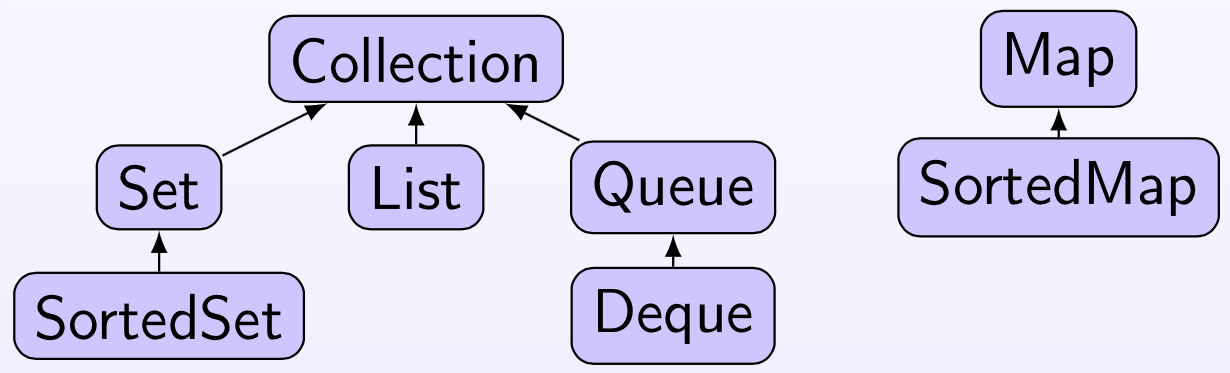
\includegraphics[width=0.5\textwidth]{colls-coreInterfaces.png}
    \label{Fig:collections}
  \caption{Interfacce del  Java collection framework.}
\end{figure}
Ogni interfaccia \`e generica. Quando dichiari una collezione devi specificare il tipo degli oggetti contenuti nella collezione. Questo permette al compilatore di verificare \textbf{a compile time} che l'oggetto che inserisci all'interno delle collezioni \`e corretto. 
\begin{lstlisting}
 Collection<String> mazzo=...
\end{lstlisting}
\end{frame}
%
%
\begin{frame}[fragile]
\frametitle{Interfacce}
Di seguito vengono specificate le interfacce principali
\begin{itemize}
\item \texttt{Collection}: 
\begin{itemize}
\item rappresenta un gruppo di oggetti (i suoi elementi). 
\item L'interfaccia collection \`e la pi\`u generale. Va utilizzata quando un livello massimo di generalit\`a \`e richiesto. 
\item   Non esiste una classe cheimplementa direttamente collection. 
\end{itemize}
\item \texttt{Set}: 
\begin{itemize}
\item una collezione che \textbf{non} pu\`o contenere elementi duplicati.
\item Consente di modellare entit\`a come per esempio un mazzo di carte da briscola (perch\`e non \`e adatto per un mazzo di carte da scala?) l'insieme di esami sostenuti da uno studente, i processi in esecuzione su una macchina.
\end{itemize} 
\item \texttt{SortedSet}: 
\begin{itemize}
\item un \texttt{Set} che mantiene gli elementi ordinati in ordine ascendente.  
\item \texttt{SortedSet} possono essere utilizzati (per esempio) per memorizzare una lista ordinata di parole.
\end{itemize}
\end{itemize}
\end{frame}
%
\begin{frame}[fragile]
\frametitle{Interfacce}
\begin{itemize}
\item \texttt{List}: 
\begin{itemize}
\item \`e una collezione ordinata (a volte chiamata sequenza)
\item Una lista pu\`o contenere elementi duplicati. 
\item L'utilizzatore di una lista vuole un controlllo preciso su dove un elemento \`e inserito e vuole potervi accedere in base alla loro posizione. \item Pu\`o essere utile al fine di modellizzare l'ordine di arrivo a un gran premio di formula 1.
\end{itemize} 
\item \texttt{Queue}: 
\begin{itemize}
\item \`e una collezione utilizzata per modellizzare una coda di elementi  prima che vengano processati. 
\item Una coda \`e in genere implementata con una FIFO 
\item Consente di eseguire operazioni come l'inserimento, l'estrazione o l'ispezione. 
\item pu\`o essere utilizzata per modellare le macchine in coda in un casello autostradale.
\end{itemize}
\item \texttt{Deque}: 
\begin{itemize}
\item A differenza della coda, \`e possibile aggiungere e rimuovere gli elementi da entrambi i lati.
\end{itemize} 
\end{itemize}
\end{frame}

\begin{frame}[fragile]
\frametitle{Interfacce}
\begin{itemize}
\item \texttt{Map}:
\begin{itemize}
\item  \`e un oggetto che mappa una chiave in un valore.
\item  Una mappa \textbf{non} pu\`o contenere delle chiavi duplicate, ogni chiave deve essere associata a esattamente un valore (che potrebbe essere un \textbf{Set}). 
\end{itemize}
\item \texttt{SortedMap}:
\begin{itemize}
\item contiene una mappa dove le chiavi sono mantenute in ordine ascendente. 
\item le mappe ordinate possono essere utilizzate per modellizzare un vocabolario o una guida telefonica.
\end{itemize}
\end{itemize}
\end{frame}



\subsection{Implementazioni}
\begin{frame}[fragile]
\frametitle{Implementazioni}
Abbiamo varie implementazioni per vari contesti, tra le quali:
\begin{itemize}
\item \texttt{Implementazioni General-purpose} sono quelle comunemente utilizzate, progettate per l'uso di tutti i giorni
\item \texttt{Implementazioni Special-purpose} sono progettati per usi particolari: garantire performances particolari, restringere l'utilizzo di quelle general purpose.
\item \texttt{Concurrent implementations} sono progettate per supportare applicazioni concorrenti. Queste implementazioni fanno parte del  java.util.concurrent package.
\item \texttt{Wrapper implementations} sono utilizzate in combinazioni con altri tipi di implementazioni per fornire funzionalit\`a aggiunte o ristette.
\end{itemize}
\end{frame}
%

\begin{frame}[fragile]
\frametitle{Implementazioni}
Le implementazioni General-purpose sono schematizzate nella tabella seguente 
\begin{table}[!ht]
{\footnotesize
\begin{tabular}{ | l | l | l | l | l | l |}
\hline
  Interfaces & Hashtable  & Resizable array  & Tree  & Linked list  & \pbox{20cm}{Hash table \\ + Linked list}  \\
  \hline
  \texttt{Set} & \texttt{HashSet} &  & \texttt{TreeSet} && \texttt{LinkedHashSet} \\
  \hline
    \texttt{SortedSet} & &  & \texttt{TreeSet} &&  \\
  \hline
  \texttt{List} &  & \texttt{ArrayList}  & & \texttt{LinkedList} & \\
\hline  
  \texttt{Queue} &  & & & \texttt{LinkedList} &  \\
\hline  
  \texttt{Deque} &  & \texttt{ArrayDeque} & & \texttt{LinkedList} & \\
\hline  
  \texttt{Map} & \texttt{HashMap} & & \texttt{TreeMap} && \texttt{LinkedHashMap} \\
  \hline
    \texttt{SortedMap} & & & \texttt{TreeMap} &&  \\
\hline    
\end{tabular} }
\end{table}
\end{frame}

\begin{frame}[fragile]
\frametitle{Implementazioni}
Ognuna di queste implementazioni:
\begin{itemize}
\item permette elementi \texttt{null} (sia per chiavi che per valori)
\item non \`e sincronizzata (thread-safe): non adatta quando thread concorrenti devono modificare la collezione
\item ha degli itaratori \emph{fail-fast} lanciano un eccezione quando viene eseguita una modica durante un iterazione. 
\item sono tutte serializzabili
\item hanno tutte un metodo clone (nota il metodo clone non clona gli elementi ma solo i loro references)
\end{itemize}
\end{frame}

\begin{frame}[fragile]
\frametitle{Implementazioni}
\begin{framed}
Come regola \`e bene pensare in termini di interfacce e non di implementazioni. 
\begin{itemize}
\item Nella maggior parte dei casi l'implementazione influenza solo le performances. 
\item \`E bene associare un implementazione direttamente alla sua interfaccia e specificare come parametri di ingresso o uscita dei metodi solamente interfacce, lasciando il programmatore libero di cambiare implementazione a suo piacimento. 
\end{itemize}
\end{framed}
\end{frame}
%
%
%%------------------------------------------------


\subsection{Collection}
\begin{frame}[fragile]
\frametitle{Interfacce: collection}
\begin{itemize}
\item \texttt{boolean	containsAll(Collection<?> c)}: Returns true if this collection contains all of the elements in the specified collection.
\item \texttt{addAll(Collection<? extends E> c)}: Adds all of the elements in the specified collection to this collection (optional operation).
\item \texttt{removeAll(Collection<?> c)}: Removes all of this collection's elements that are also contained in the specified collection (optional operation).
\item \texttt{retainAll(Collection<?> c)}: Retains only the elements in this collection that are contained in the specified collection (optional operation).
\item \texttt{clear()}: Removes all of the elements from this collection (optional operation).
\end{itemize}
\end{frame}


\subsection{Conversione tra collezioni}
\begin{frame}[fragile]
\frametitle{Conversione tra collezioni}
Ogni collezione ha un costruttore (detto \emph{conversion constructor}) che prende come parametro una collezione. \`E possibile usare questo costruttore per convertire una collezione di un tipo in un'altra collezione di un altro tipo.
\begin{lstlisting}
List<String> ls=new ArrayList<String>();
Set<String> lo=new HashSet<String>(ls);
\end{lstlisting}
\end{frame}

\subsection{Conversione tra array e collezioni}
\begin{frame}[fragile]
\frametitle{Conversione tra collezioni}
\begin{itemize}
\item da collection a array: per convertire un array in una collezione \`e possibile utilizzare il metodo \texttt{toArray()} specificata nell'interfaccia \texttt{List}
\begin{lstlisting}
List<String> miaLista=new ArrayList<String>();
String[] array=miaLista.toArray();
\end{lstlisting}
\end{itemize}
\begin{itemize}
\item da array a collection: per convertire da un array a una collezione si pu\`o utilizzare il metodo \texttt{statico} \texttt{asList} della classe \texttt{Array}.
\begin{lstlisting}
String[] stringArray = new String[20];
List<String> miaList=Arrays.asList(stringArray);
Set<String> mioSet=new HashSet<String>(miaList);
\end{lstlisting}
\end{itemize}
\end{frame}

\subsection{Iterazione}
\begin{frame}[fragile]
Per eseguire delle iterazioni su una collezione ci sono due possibili modi:
\begin{itemize}
\item for generalizzato:
\begin{lstlisting}
Collection<String> collezione=new HashSet<String>();
for(String s: collezione){
    System.out.println(s);
}
\end{lstlisting}
\item iteratore:
\begin{lstlisting}
Collection<String> collezione=new HashSet<String>();
Iterator<String> it=c.iterator;
while(it.hasNext()){
    System.out.println(it.next());
}
\end{lstlisting}

\end{itemize}

\end{frame}





\subsection{Esercizio 1 (assegnamenti)}
\begin{frame}[fragile]
\frametitle{Esercizio 1}
\begin{framed}
\textbf{Esercizio 1}: Dire se sono valide le seguenti operazioni
\begin{lstlisting}
List<String> ls=new ArrayList<String>();
List<Object> lo=ls;
\end{lstlisting}
\end{framed}
\end{frame}

\begin{frame}[fragile]
\frametitle{Esercizio 1}
\begin{lstlisting}
List<String> ls=new ArrayList<String>(); // certamente si
List<Object> lo=ls;    //no, il compilatore non lo permette
\end{lstlisting}
\end{frame}



\subsection{Esercizio 2 (Rimozione di duplicati)}
\begin{frame}[fragile]
\frametitle{Esercizio 2: rimozione duplicati}
\begin{framed}
\textbf{Esercizio 2}: Scrivere un metodo statico che data una collezione di \texttt{String} rimuove i duplicati e stampa il numero di elementi non duplicati e i corrispettivi elementi
\end{framed}
\end{frame}

\begin{frame}[fragile]
\frametitle{Esercizio 2: rimozione duplicati}
Nella prima versione della soluzione utilizziamo il for generalizzato
\begin{framed}
\begin{lstlisting}
public class FindDups {
    public static void findDups(Collection<String> words){
	    Set<String> set = new HashSet<String>();
	    for (String s: words){
	        set.add(s);
	    }
	    System.out.println("Unique values, dim : " + 
		set.size() + " Elements:" + set);
	}
}
\end{lstlisting}
\end{framed}
\end{frame}

\begin{frame}[fragile]
\frametitle{Esercizio 2: rimozione duplicati}
Nella seconda versione utilizziamo direttamente il costruttore di \texttt{HashSet} vedi (\url{https://docs.oracle.com/javase/6/docs/api/java/util/HashSet.html})
\begin{framed}
\begin{lstlisting}
public class FindDups {
    public static void findDups(
                Collection<String> words){
        Set<String> set = new HashSet<String>(words);
        System.out.println("Unique values, dim : " + 
            set.size() + " Elements:" + set);
       }
}
\end{lstlisting}
\end{framed}
\end{frame}

\subsection{Esercizio 3 (Shuffle)}
\begin{frame}[fragile]
\frametitle{Esercizio 3: Shuffle}
\begin{framed}
\textbf{Esercizio 3}: Scrivere un metodo statico che data una lista permette di mescolare degli oggetti contenuti in una lista.
\end{framed}
\end{frame}

\begin{frame}[fragile]
\frametitle{Esercizio 3: Shuffle}
\begin{framed}
\begin{lstlisting}
public class Shuffle {
    public static <E> void swap(List<E> a, int i, int j) {
        E tmp = a.get(i);
        a.set(i, a.get(j));
        a.set(j, tmp);
   }
   public static void shuffle(List<Integer> list, 
       Random rnd) {
       for (int i = list.size(); i > 1; i--)
           swap(list, i - 1, rnd.nextInt(i));
      }
}
\end{lstlisting}
\end{framed}
\end{frame}


\begin{frame}[fragile]
\frametitle{Esercizio 3: Shuffle}
\begin{framed}
\begin{lstlisting}
public class Shuffle {
    public static void shuffle(List<Integer> list) {
        Collections.shuffle(list);
    }
}
\end{lstlisting}
\end{framed}
\end{frame}

\subsection{Esercizio 4 (number of Tokens)}
\begin{frame}[fragile]
\frametitle{Esercizio 4: number of Tokens}
\begin{framed}
\textbf{Esercizio 4}: Scrivere un metodo statico che data una stringa conta il numero di occorrenze di ogni parola. Suggerimento: controllare la Javadoc della classe \texttt{StringTokenizer}
\end{framed}
\end{frame}

\begin{frame}[fragile]
\begin{framed}
\begin{lstlisting}
public static void count(String text){
    StringTokenizer tokenizer = 
        new StringTokenizer(text);
    Map<String,Integer> frequencyCounterMap = 
        new HashMap<String,Integer>();
    while (tokenizer.hasMoreTokens()){
        String word = tokenizer.nextToken();
        Integer freq = frequencyCounterMap.get(word);
        frequencyCounterMap.put(word,
            (freq == null) ? 1 : freq + 1);
    }
    System.out.println(frequencyCounterMap.size() +
         " parole distinte");
    System.out.println(frequencyCounterMap);
}
\end{lstlisting}
\end{framed}
\end{frame}


\subsection{Esercizio 5: Scrivere un metodo che stampa gli elementi di una collection di qualsiasi tipo.}
\begin{frame}[fragile]
\frametitle{WildCard}
\begin{framed}
Esercizio 5: Scrivere un metodo che stampa gli elementi di una collection di qualsiasi tipo.
\end{framed}
\end{frame}


\begin{frame}[fragile]
\frametitle{WildCard}
La prima soluzione che potrebbe venirci in mente \`e la seguente: dichiarare un metodo che prende come parametro una collezione di elementi il cui tipo \`e \texttt{Object}.
\begin{framed}
\begin{lstlisting}[language=Java]
void printCollection(Collection<Object> c){
    for(Object e: c){
        System.out.println(e);    
    }
}
\end{lstlisting}
\end{framed}
 Tuttavia questa soluzione non ci pemette di stampare una collezione di \texttt{String}. Infatti, bench\`e \texttt{String} estende \texttt{Object} non \`e vero che \texttt{Collection<Object>} estende \texttt{Collection<String>}. Quindi non \`e possibile chiamare il metodo \texttt{printCollection} passando come parametro una \texttt{Collection<String>}.
\end{frame}
%
\begin{frame}[fragile]
\frametitle{WildCard}
\begin{framed}
\begin{lstlisting}[language=Java]
void printCollection(Collection<?> c){
    for(Object e: c){
        System.out.println(e);    
    }
}
\end{lstlisting}
\end{framed}
\end{frame}

\subsection{Esercizio 6: Bounded Wildcard}
\begin{frame}[fragile]
\frametitle{Bounded Wildcard}
\begin{framed}
Esercizio 6: Aggiungere un metodo \texttt{drawAll} in ShapeClient per disegnare tutte le figure di una lista di figure
\end{framed}
\end{frame}


\begin{frame}[fragile]
\frametitle{Bounded Wildcard}
	La prima soluzione a cui possiamo pensare \`e la seguente:
	\begin{framed}
	\begin{lstlisting}
	void drawAll(List<Shape> shapes) { 
	    for (Shape s : shapes) {
	        s.draw(this); 
	    }
	}
	\end{lstlisting}
\end{framed}
\end{frame}

\begin{frame}[fragile]
\frametitle{Bounded Wildcard}
\begin{framed}
\begin{lstlisting}
void drawAll(List<? extends Shape> shapes) { 
    for (Shape s : shapes) {
        s.draw(this); 
    }
}
\end{lstlisting}
\end{framed}
\end{frame}

%-------------

%------------------------------------------------


%----------------------------------------------------------------------------------------

\end{document} 
%
%\documentclass{beamer}
%\usepackage[english]{babel}
%\usepackage{xcolor}
%\usepackage[utf8]{inputenc}
%%\usepackage[ngerman]{babel}
%\usepackage{hyperref}
%\usepackage{graphicx}
%\usepackage{listings} % Required for insertion of code
%%\usepackage[pdftex]{color}
%%\usepackage{colortbl}
%%\usepackage{listings}
%\usepackage{xcolor}
%\usepackage[lf]{venturis}
%\usepackage{amsmath}
%\usepackage{amsfonts}
%\usepackage{amssymb}
%\usepackage{subcaption}
%%\usepackage{multirow}
%\usepackage[version=3]{mhchem}
%%\usepackage{longtable}
%\usepackage{pgf}
%\usepackage{tikz}
%\usepackage[citetracker=true,sorting=none,backend=bibtex,autocite=footnote]{biblatex}
%{\fontsize{2}{2} \bibliography{bibliography}}
%
%\renewcommand{\bibfont}{\tiny}
%
%\definecolor{kugreen}{RGB}{6,76,149}
%\definecolor{kugreenlys}{RGB}{132,158,139}
%\definecolor{kugreenlyslys}{RGB}{173,190,177}
%\definecolor{kugreenlyslyslys}{RGB}{214,223,216}
%\setbeamercovered{transparent}
%
%
%
%
%
%
%\setbeamertemplate{navigation symbols}{}
%
%  
%\mode<presentation>
%{  \usetheme{Madrid}
%  \usecolortheme[named=kugreen]{structure}
%  \useinnertheme{circles}
%  \usefonttheme[onlymath]{serif}
%  \setbeamercovered{transparent}
%  \setbeamertemplate{blocks}[rounded][shadow=true]
%}
%
%
%
%
%%\setbeamerfont{myTOC}{series=\bfseries}
%\AtBeginSection[]{\frame{\frametitle{Outline}%
%                  \usebeamerfont{myTOC}\tableofcontents[current]}}
%                  
%\title[Agile Verification]{Agile Verification}
%\author[C. Menghi]{Student: Claudio Menghi \\ Supervisor: Carlo Ghezzi}
%\institute[]{Politecnico di Milano}
%\date{29 October 2014}
%
%\begin{document}
%\frame{
%\titlepage \vspace{-0.5cm}
% }
%
%
%\frame
%{
%\frametitle{Overview}
%\tableofcontents[]
%}
%

%
%
%%\section*{Bibliography}
%%\begin{frame}[allowframebreaks]{Bibliography}
%%\footnotesize{
%%\bibliographystyle{abbrv}
%%\bibliography{bibliography} }
%%\end{frame}
%
%\end{document}
